\documentclass{beamer}
\usetheme{CambridgeUS}
\usecolortheme{beaver}

\title[GJK]{Gilbert-Johnson-Keerthi Algorithm}
\author{Minliang LIN}
\date{\today}

% control sequence whose name is non-letter
% doesn't require either spaces or braces aftet it
\def\*#1{\mathbf{#1}}
\newcommand{\norm}[1]{\left\lVert#1\right\rVert}
% \usepackage{listings}
\usepackage[export]{adjustbox}

\begin{document}
% adjust math displaystyle
\everymath{\displaystyle}

\begin{frame}
  \titlepage
\end{frame}

\begin{frame}
  \frametitle{Outline}
  \tableofcontents
\end{frame}

\section{Introduction}
\begin{frame}
\frametitle{Minimum distance of two convex sets}
  \begin{itemize}
    \item $ minDistance(A, B) = min\{\norm{a - b} \mid a\in A, b\in B\}$
  \end{itemize}
  \begin{columns}
    \column[]{0.5\textwidth}
    \centering
    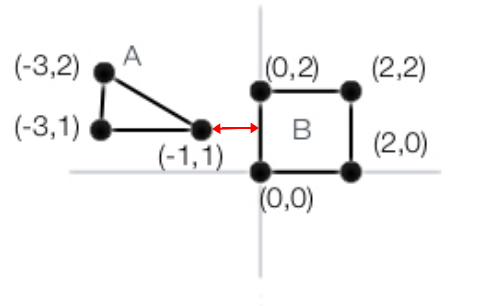
\includegraphics[width=0.7\textwidth]{images/g1}\\
    min distance = 1
    \column[]{0.5\textwidth}
    \centering
    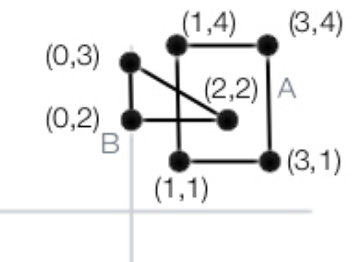
\includegraphics[width=0.7\textwidth]{images/g2}\\
    min distance = 0
  \end{columns}
\end{frame}

\begin{frame}
\frametitle{Minkowski Sum}
  \begin{itemize}
    \item<1-> $ C = A + (-B) = \{a - b|a\in A, b\in B\} $
    \item<2-> $ minDistance(A, B) = min\{\norm{c} \mid c \in C\} $
  \end{itemize}
  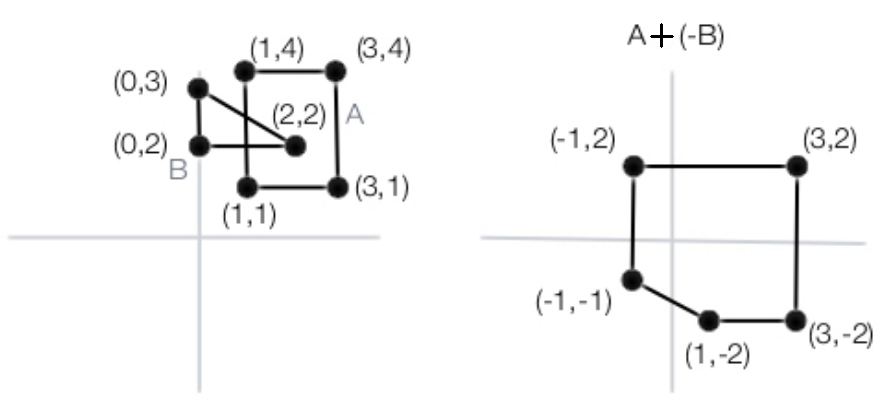
\includegraphics[width=0.7\textwidth]{images/g3}
\end{frame}

\begin{frame}
\frametitle{The Main Idea of GJK for \textbf{Collision Detection}}
  \only<1>{
    \begin{itemize}
      \item
        Try to enclose the origin with a triangle/tetrahedron/line/point(i.e. simplex) $\tau_k\subseteq C$ iteratively.
      \item $min\norm{t}\approx min\norm{c}, t\in\tau_k, c\in C$.
    \end{itemize}
    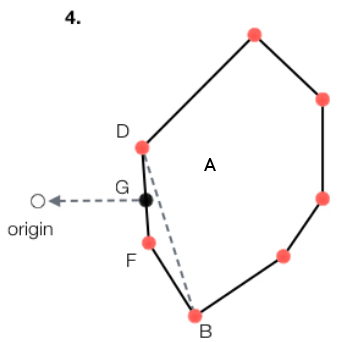
\includegraphics[width=0.4\textwidth, right]{images/g8}
  }
  \only<2>{
    \begin{itemize}\item{
    Given set $A$ and direction $d$, $Support(A, d) = \{s|s\in A, s\cdot d = max\{w\cdot d \mid w \in A\}\}$
    }\end{itemize}
    \raggedright
    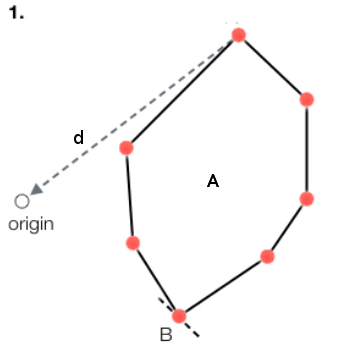
\includegraphics[width=0.4\textwidth, right]{images/g9}
  }
\end{frame}

\begin{frame}[fragile]% for lstlisting is a kind of verbatim
\frametitle{The Main Idea of GJK for \textbf{Collision Detection}}
  \begin{columns}
    \column[]{0.5\textwidth}

%%source code indent
{\tiny
\begin{verbatim}
S = Support(C, random_direction)
[] = S
D = -S
Loop:
  S = Support(C, D)
  If dot(S, D) < 0:
    NO INTERSECTION, BREAK
  [] += S
  [], D, contains_origin = NearestSimplex([])
  If contains_origin
    INTERSECTION, BREAK
\end{verbatim}
}

    \column[]{0.5\textwidth}
      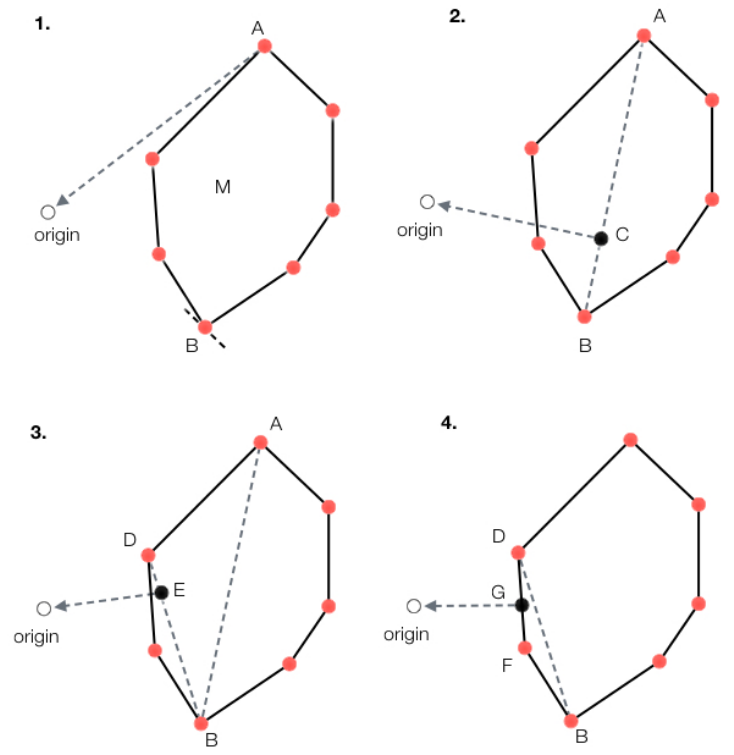
\includegraphics[width=\textwidth]{images/g7}
  \end{columns}
\end{frame}

\begin{frame}
\frametitle{Finding Support}
  Simple for polytope:\\
  $Support(A+(-B), d) = Support(A, d)-Support(B, -d)$\\
  If $A$ is $m$-polytope, $B$ is $n$-polytope. Finding support is $O(m+n)$.\\
  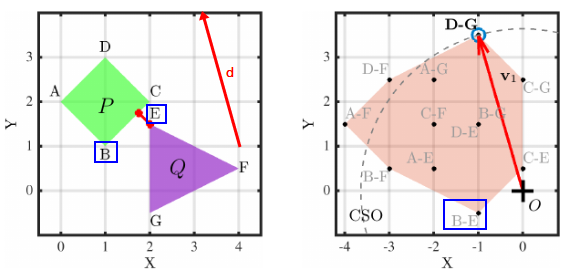
\includegraphics[width=0.8\textwidth]{images/g10}
\end{frame}

\begin{frame}
\frametitle{Update Simplex and Direction}
  \begin{columns}
    \column[]{0.5\textwidth}
      Given simplex $\tau$ and direction $d$.
      \begin{itemize}
        \item<1> Enumerate all Voronoi region to locate the origin
        \item<2> Different enumerative method
        \item<3>{
          My understanding: minimum square or projection.
          \begin{itemize}
            \item If $O \in \tau$, return INTERSECTION
            \item Else update the direction
          \end{itemize}
        }
      \end{itemize}
    \column[]{0.5\textwidth}
    \centering
    \includegraphics<1>[width=\textwidth]{images/g11}
    \includegraphics<2>[width=0.5\textwidth]{images/g12}\\
    \includegraphics<2>[width=0.5\textwidth]{images/g13}
  \end{columns}
\end{frame}

\end{document}
